\documentclass[a4paper, 11pt, oneside]{article}

\newcommand{\plogo}{\fbox{$\mathcal{PL}$}} 
\usepackage{amsmath}
\usepackage[utf8]{inputenc} 
\usepackage[T1]{fontenc} 
\usepackage{enumitem}
\usepackage{graphicx}
\usepackage{graphicx}
\usepackage{supertabular}
\usepackage{hyperref}
\usepackage[spanish]{babel}
\graphicspath{{Imagenes/}}

\begin{document} 

\begin{titlepage} 

	\centering 
	
	\scshape 
	
	\vspace*{\baselineskip} 
	
	
	
	\rule{\textwidth}{1.6pt}\vspace*{-\baselineskip}\vspace*{2pt} 
	\rule{\textwidth}{0.4pt} 
	
	\vspace{0.75\baselineskip} 
	
	{\LARGE Parcial 2: AntiX}	
	\vspace{0.75\baselineskip} 
	
	\rule{\textwidth}{0.4pt}\vspace*{-\baselineskip}\vspace{3.2pt}
	\rule{\textwidth}{1.6pt} 
	
	\vspace{2\baselineskip} 
	

	ADMINISTRACIÓN DE SISTEMAS UNIX/LINUX
	
	\vspace*{1\baselineskip} 
	
	
	
	Alumna:
	
	\vspace{0.2\baselineskip} 
	
	{\scshape\Large Karla Adriana Esquivel Guzmán}  
	\vspace{0.5\baselineskip} 
	\vfill
	
\includegraphics{unam.jpg}
	
	\textit{UNIVERSIDAD NACIONAL AUTONOMA DE MEXICO} 
	
	
	
	
	
	\vspace{0.3\baselineskip} 
	
	30/Abril/2019 
	
	 

\end{titlepage}

\section*{Distribución}
La distribución de Linux que elegí es \textbf{antiX}, en principio es de las distribuciones que te facilitan bajar el .iso de versiones viejas, la comparación que hago en éste reporte es entre la versión \textbf{antiX-M7.2} y la última versión que hay hasta ahora \textbf{antiX-17.4.1}.

\section*{Comparación}
\section*{antiX-M7.2:}
\begin{itemize}
    \item El tiempo de descarga fue de 1m 36.511s
    \begin{center}
        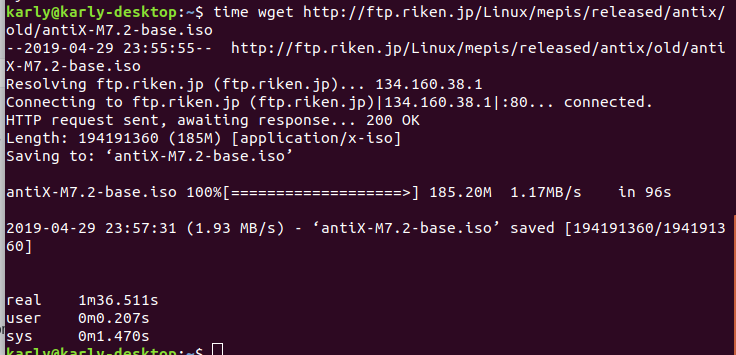
\includegraphics[scale=0.45]{antix2.png}
    \end{center}
    \item El tamaño de la imagen \.iso es de 194.2 MB
    \item Empezando por la instalación, utilicé la opción de instalación predeterminada, desde un inicio se notó la diferencia entre versiones pues en ésta no contaba con entorno gráfico, aunque su instalación es muy sencilla, y al entrar si quieres agregar una contraseña simplemente escribes el comando \textbf{passwd} y sin problema puedes agregar una contraseña.
    
    \begin{center}
        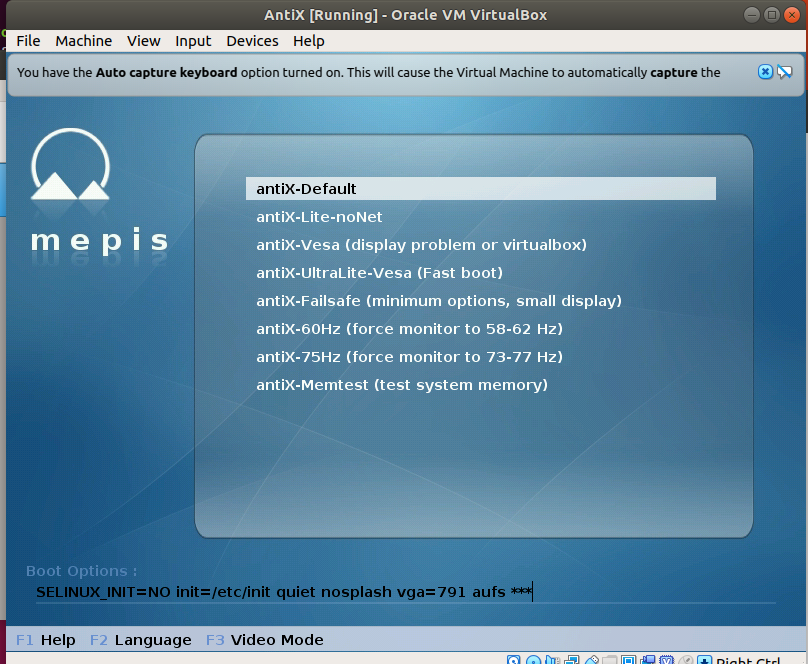
\includegraphics[scale=0.40]{instalacion1.png}
    \end{center}
    
    \item En el directorio principal hay varias diferencias, distintas carpetas en ambas distribuciones, incluido que en ésta versión de antiX hay una carpeta llamada \textbf{cdrom}, investigando un poco encontré lo siguiente sobre ésta carpeta(folder): Al igual que el directorio 
    $/floppy$, el uso del directorio $/cdrom$, puede montar discos en cualquier directorio vacío que se deseé. (Incluso se podría, por ejemplo, montar discos de la unidad de CD-ROM en / disquete y montar disquetes en / cdrom, aunque esto a mi parecer ya es algo obsoleto para estos tiempos modernos en que las computadoras ya ni siquiera tienen unidad de CDROM).
    
    \item También se encuentra la carpeta ramdisk, que ya no se encuentra en la versión más nueva de antiX, \textbf{ramdisk} es un sistema de archivos raíz inicial que se monta antes de que el sistema de archivos raíz real esté disponible, está vinculado al kernel y se carga como parte del procedimiento de arranque del kernel. 
    
    \item Otra Carpeta que se encuentra en ésta versión y no en la más actual es \textbf{aufs}, éste es un sistema de archivos de unión. El controlador de almacenamiento aufs era anteriormente el controlador de almacenamiento predeterminado utilizado para administrar imágenes y capas en Docker para Ubuntu, y para las versiones Debian anteriores a Stretch.
    
    
    \begin{center}
        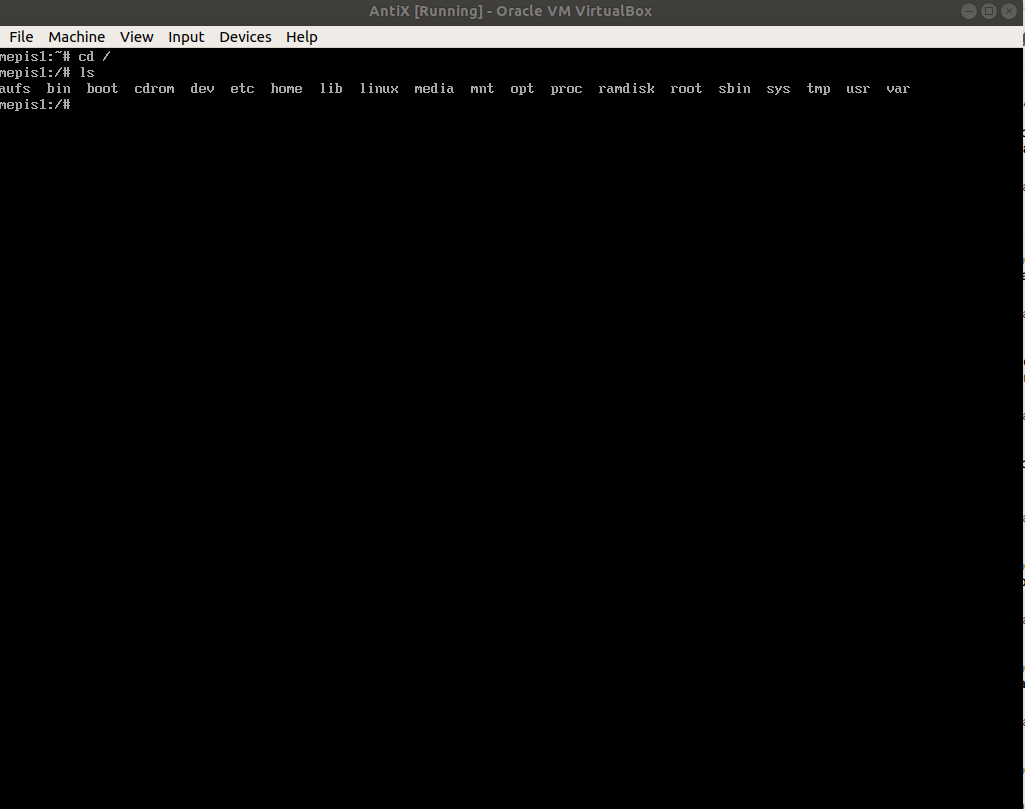
\includegraphics[scale=0.32]{antix3.png}
    \end{center}
    
     \textbf{KERNEL:} La versión del kernel es 2.6.22-1-mepis-smp, además en el directorio /sys/kernel
     ésta versión tiene únicamente 3 carpetas, security, uevent\_helper y uevent\_seqnum.
\end{itemize}
\section*{antiX-17.4.1:}
\begin{itemize}
    \item El tiempo de descarga fue de 4m 24.596s
    \begin{center}
        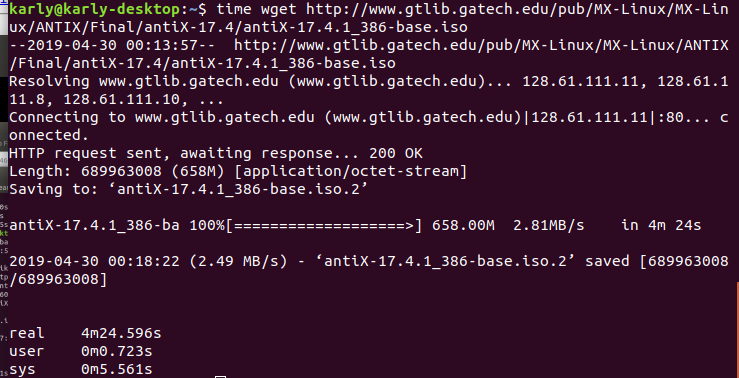
\includegraphics[scale=0.44]{antix1.png}
    \end{center}
    \item Ésta versión no es menos sencilla de instalar que la más vieja, de hecho la versión por default ya cuenta con entorno gráfico que de hecho es muy amigable a la vista y fácil de utilizar. Aunque en esta versión ya existe una contraseña por default para entrar en modo super usuario, la cual es "demo".
    
    \begin{center}
        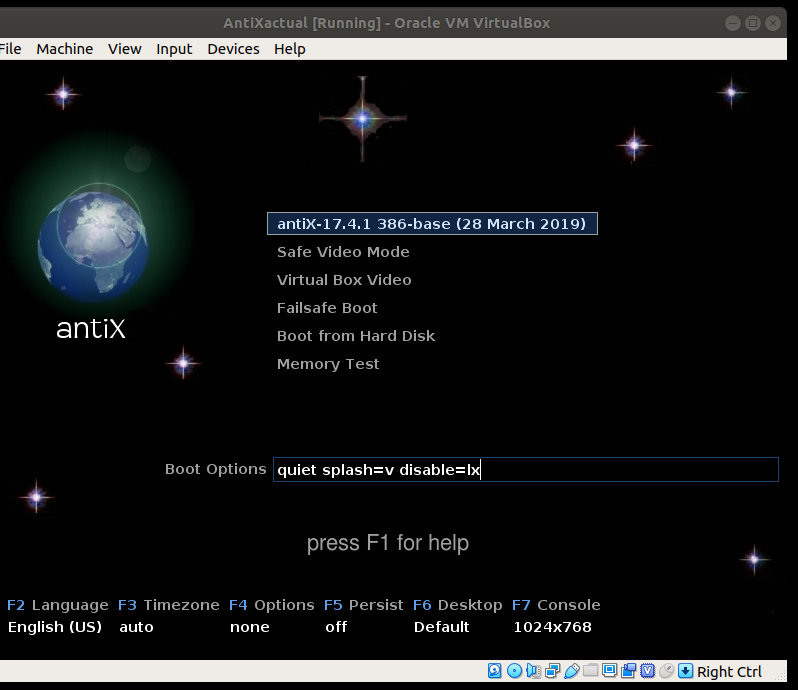
\includegraphics[scale=0.40]{instalacion2.png}\\
        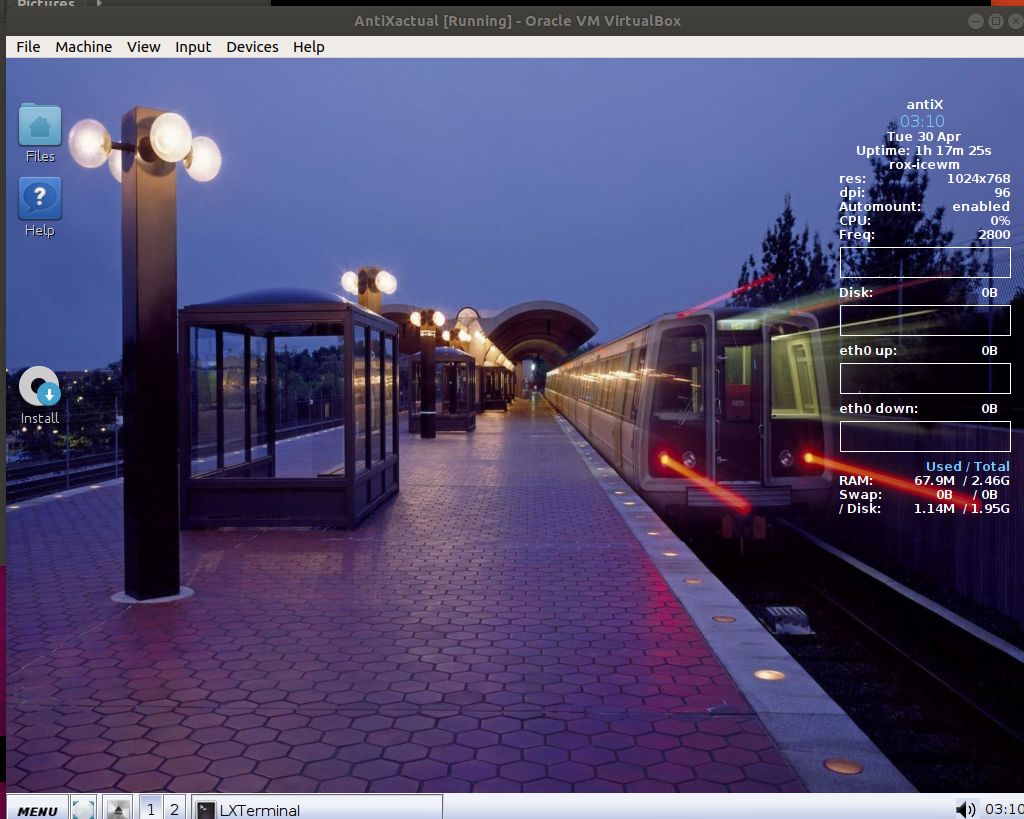
\includegraphics[scale=0.32]{instalacion3.png}
    \end{center}
    \item El tamaño de la imagen \.iso es de 690.0 MB
    \item Ésta versión de antiX además del directorio $/cdrom$ también tiene el directorio $/mnt$ que básicamente cumple con las mismas funciones es un "punto de montaje".
    
    
    \begin{center}
        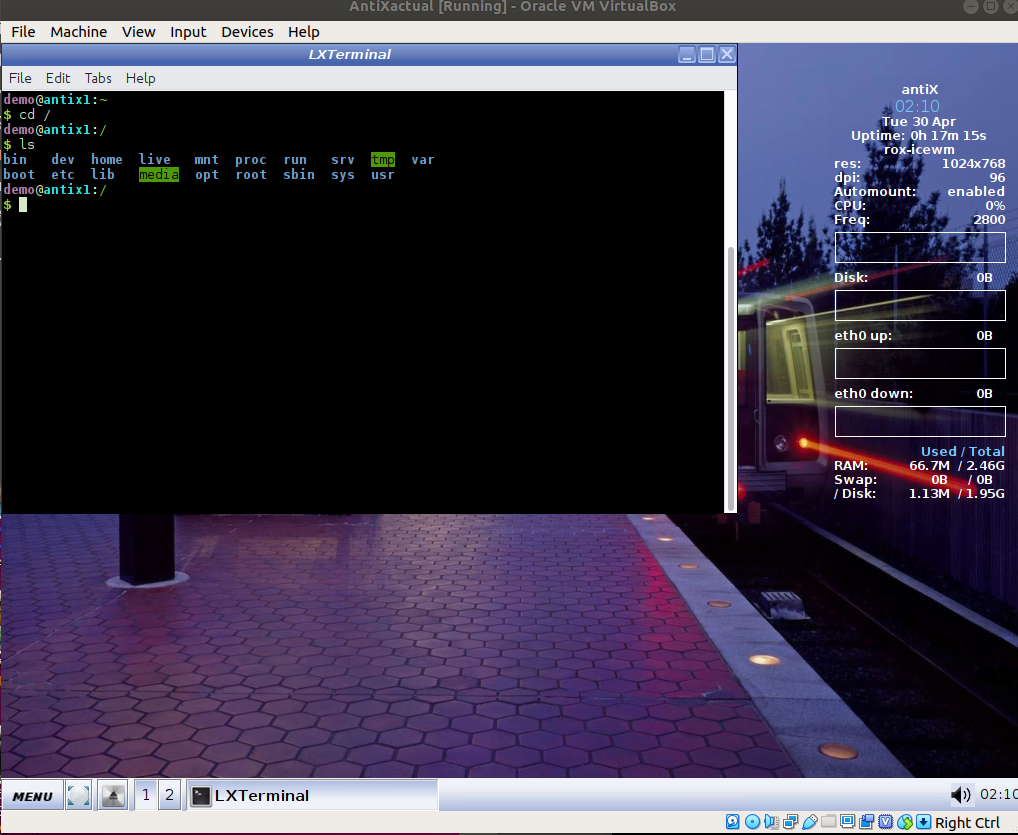
\includegraphics[scale=0.30]{antix4.png}
    \end{center}
    
     \textbf{KERNEL:} La versión del kernel es 4.9.160-antix.2-486-smp, ésta versión a diferencia de la más vieja, cuenta con las carpetas boot\_params, debug, fscaps, iommu\_groups, irq, kexec\_crash\_loaded, kexec\_crash\_size, kexec\_loaded, mm, notes, rcu\_expedited, rcu\_normal, security, slab, tracing, uevent\_helper, uevent\_seqnum y vmcoreinfo.
     
     \begin{center}
         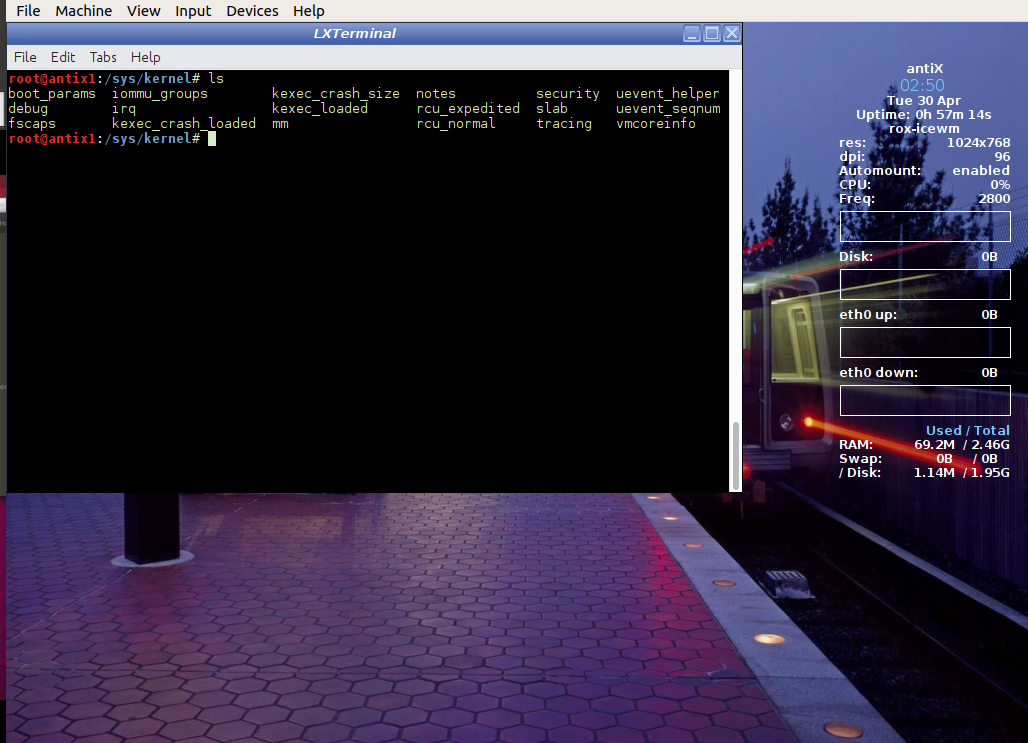
\includegraphics[scale=0.30]{antix6.png}
     \end{center}
\end{itemize}
\section*{CONCLUSIÓN:}
En conclusión el sistema de archivos ha cambiado de manera considerable, igual que los recursos que el sistema operativo requiere, aunque hasta la fecha antiX es un sistema operativo súper ligero y amigable para instalar en computadoras con pocos recursos, de manera personal me gusta mucho el entorno gráfico de la última versión. La versión antiX-M7.2 me recuerda mucho a Minix, el directorio raíz se le parece mucho. Fuera de las diferencias en el entorno gráfico, versión del kernel, tamaño, etcétera, me parece que en ambas versiones puede trabajarse bastante bien y casi no se nota la diferencia entre una y otra para usuarios que ya tenemos experiencia utilizando Linux y estamos acostumbrados a trabajar con o sin un entorno gráfico.
\end{document}